\section{Equal-budget UC follow-up}\label{app:uc-equal-compute}
The equal-budget follow-up asks whether structural UC supervision improves selective-set recovery over direct membership heads when each complete system receives the same training and development allocation. It uses fresh collections and a prospectively frozen protocol, without external preregistration. Its two primary comparisons remain separate from the matched-epoch study's three-comparison family (Appendix~\ref{app:ibm-gpu}). The operators, observation model, generators, pair estimator, and optimizer are unchanged. This experiment concerns UC only.

\subsection{Data, objectives, and native readouts}
A separate frozen root seed defines twelve independent collections. Each contains 512 training and 128 development graphs at $n=12$, with 256 held-out graphs at each $n=24$ and $n=48$. The ordered, planted, separated, rank-mixture, and random families cycle by graph index as in Appendix~\ref{app:ibm-gpu}. The same count intensity 10, planned pair missingness 0.25, tie probability 0.20, and heterogeneous count construction apply. Latent graphs have strict majority relations; observation ties and missingness are retained separately in the decisive-win matrix $W$ and tied-count matrix $T$. Two independently coded hard oracles agree on the latent UC labels. All natural core classes remain in the generated data: the selective evaluation stratum is neither an acceptance rule for generating graphs nor a source of test-time cardinality information.

Three paired initializations per collection share encoder/pair parameters and epoch-specific minibatch permutations. The four complete systems are pairwise likelihood with structural UC readout; pairwise likelihood plus ordinary membership-head BCE with its direct readout; pairwise likelihood plus relational membership-head BCE with its direct readout; and pairwise likelihood plus STE UC BCE with structural readout. The relational control uses the four relation summaries, including two-step paths, described in Appendix~\ref{app:ibm-gpu}. Each supervised system considers $\lambda\in\{0.1,1\}$; pairwise-only has one candidate. Thus the run contains $12\times3\times(1+2+2+2)=252$ trained candidates and 144 selected complete systems. The pair architecture is matched, while active parameter counts differ between structural systems and direct-head systems.

Training uses Adam at 0.001, batch size 16, norm-5 gradient clipping, and the unchanged UC temperature $\tau=\gamma=0.035$. Pairwise likelihood is normalized by decisive comparisons in the minibatch; target BCE averages graphs and vertices. As in the original implementation, probabilities and BCE scores are clipped to $[10^{-6},1-10^{-6}]$ for numerical stability. This clipping can zero a saturated loss gradient and is not a modification of the mathematical operator's definition. Model inference takes only $W,T$ as inputs. Training labels supervise the appropriate losses; latent probabilities and test labels enter truth construction and diagnostic evaluation, not the prediction function.

\subsection{Charged time and development-only selection}
Each supervised system receives two 110-second candidate allocations; pairwise-only receives one 220-second allocation. Consequently every complete system receives 220 seconds per collection and initialization, totaling 31,680 allocated seconds. The charged synchronized wall clock includes training, native-readout development prediction, cutoff selection, checkpoint/development serialization, and in-loop progress bookkeeping. In particular, development evaluation of a direct-head baseline does not charge it for the unused UC operator. Data generation, initialization/data transfer, common warmup, post-budget integrity checks, and held-out evaluation are recorded outside this allocation. Equal allocation is not equal epoch count or equal update count, nor a claim of equal total application runtime.

Five checkpoints target fractions 0.025, 0.1, 0.25, 0.5, and 1 of a candidate allocation. At a synchronized minibatch boundary the scheduler reserves the largest previously measured checkpoint cost before triggering the next checkpoint; the first checkpoint has zero reserve. Evaluation and serialization count toward the same candidate budget. A prospectively fixed validity gate requires every candidate and complete-system charged total to remain within $\pm2\%$ of its allocation; a violation would withhold the confirmatory equal-budget inference. The measured charged total is 31,713.35 seconds, with maximum absolute candidate deviation 0.510\% and complete-system deviation 0.189\%. All 252 candidates and 144 systems pass, with intervening training at all five checkpoints.

Each checkpoint is calibrated on development cases with $1<|\mathrm{UC}|<12$, maximizing mean per-case F1 for its native readout. The 43 absolute cutoffs comprise $0,0.025,\ldots,1$ and the all/none sentinels $-10^{-6}$ and $1.000001$. Sets use the inclusive rule $s_a\ge h$ without an oracle-size constraint. Across candidates, ties prefer an earlier checkpoint, then smaller $\lambda$, then a cutoff nearer 0.5, then the smaller cutoff. This permits a fast baseline to select an early model rather than obliging it to use its final state. All choices for the three initializations of a collection are frozen before its held-out graphs are generated. Test outcomes choose neither $\lambda$, checkpoint, cutoff, nor operator temperature.

\subsection{Primary comparison and descriptive diagnostics}
The primary stratum is selective non-singleton UC, $1<|\mathrm{UC}|<n$, at $n=24$. For each collection and initialization, F1 first averages its eligible test graphs; the three initialization means are then averaged within the collection. The two contrasts are STE structural F1 minus ordinary auxiliary direct F1 and minus relational auxiliary direct F1. Only the twelve paired collection differences enter inference. Intervals use Student's $t_{11}$ distribution and are approximate, individual 95\% intervals rather than simultaneous intervals. The two-sided sign-flip test enumerates all $2^{12}=4096$ patterns and requires exchangeability under independent sign reversals under its null. Holm adjustment covers exactly these two contrasts. Collection independence and the approximate normality of collection differences remain relevant assumptions; individual graphs and initializations are not treated as independent replicates.

\begin{table}[ht]\centering\small
\begin{tabular}{lrrrrr}
\toprule
Objective / readout & $n$ & F1 (all) & F1 (selective) & Exact (\%) & Size \\
\midrule
Pair / structural & 24 & 0.5252 & 0.6245 & 3.76 & 16.64 \\
Pair / structural & 48 & 0.4104 & 0.4018 & 0.91 & 39.14 \\
Aux. / head & 24 & 0.5865 & 0.6414 & 3.31 & 16.57 \\
Aux. / head & 48 & 0.4633 & 0.4280 & 0.31 & 35.04 \\
Rel. aux. / head & 24 & 0.5879 & 0.6416 & 2.87 & 16.56 \\
Rel. aux. / head & 48 & 0.4651 & 0.4263 & 0.23 & 35.17 \\
STE / structural & 24 & 0.5484 & 0.6281 & 3.82 & 16.85 \\
STE / structural & 48 & 0.4276 & 0.4076 & 0.33 & 38.04 \\
\bottomrule
\end{tabular}

\caption{Complete-system UC follow-up. Each method uses its own development-selected native readout. All-class F1 uses the natural mixture; selective columns restrict to $1<|\mathrm{UC}|<n$. Exact is complete-set recovery and selected size is predicted cardinality on that stratum. Means average graphs, then three initializations, then twelve collections. Only $n=24$ selective F1 is primary.}
\label{tab:uc-equalcompute-systems}\end{table}

\begin{table}[ht]\centering\small
\begin{tabular}{lrrrrr}
\toprule
Baseline & $\Delta$ & 95\% CI & $p$ & $p_{\rm Holm}$ & Pos. \\
\midrule
Ordinary head & $-0.01329$ & $[-0.03286,+0.00628]$ & 0.1621 & 0.3193 & 5/12 \\
Relational head & $-0.01345$ & $[-0.03300,+0.00611]$ & 0.1597 & 0.3193 & 3/12 \\
\bottomrule
\end{tabular}

\caption{The two prespecified primary contrasts on selective non-singleton UC at $n=24$. Differences are STE minus the indicated direct-head system; intervals are individual paired $t_{11}$ intervals. Holm adjustment applies to the two exact sign-flip tests.}
\label{tab:uc-equalcompute-primary}\end{table}

\begin{figure}[ht]\centering
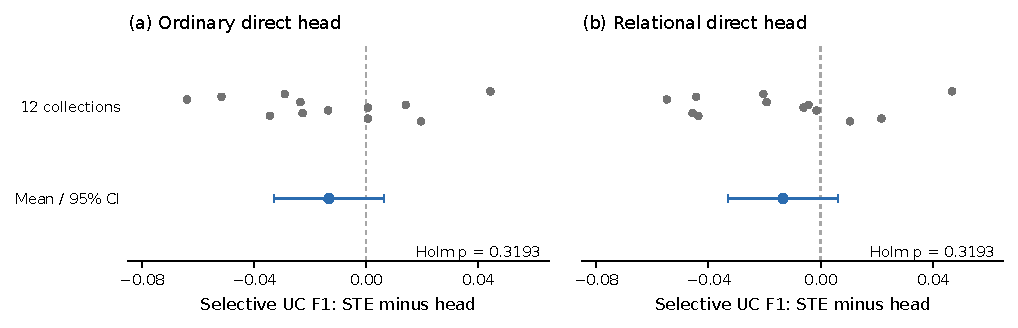
\includegraphics[width=\linewidth]{figures/v12_uc_equalcompute_effects.pdf}
\caption{All twelve independent collection differences for each primary contrast. Each small point averages the three paired initializations within one collection. The accent point and interval show the mean difference and individual, unadjusted 95\% $t_{11}$ interval. Zero marks equal mean F1; positive differences favor STE. No collection is excluded.}
\label{fig:uc-equalcompute-effects}\end{figure}

STE's primary mean F1 is 0.6281, compared with 0.6414 for the ordinary direct head and 0.6416 for the relational direct head. Corresponding differences are $-0.01329$ (95\% interval $[-0.03286,0.00628]$) and $-0.01345$ ($[-0.03300,0.00611]$); both Holm-adjusted $p$-values are 0.3193. STE has positive collection differences in five of twelve ordinary-head comparisons and three of twelve relational-head comparisons. This study therefore does not demonstrate an equal-budget STE advantage over either direct-head baseline. Negative point estimates do not establish inferiority; intervals crossing zero do not establish equivalence or noninferiority. The earlier common-structural-readout, matched-epoch result concerns a different comparison and does not resolve this complete-system question. Compute allocation, baseline readout, development criterion, and primary stratum differ between studies; their change in outcomes cannot be attributed to compute alone.

The $n=48$ results, mixed-class averages, singleton/full-core strata, exact recovery, cardinalities, AP/AUROC, pairwise-only control, and generator breakdowns are descriptive secondary outputs. AP/AUROC are defined only when both positive and negative reference memberships exist, so their support differs from F1. The explicit all/none predictions are constant controls, not trained methods. Saved predicted pair matrices permit additional diagnostics of relation quality, independently of development-selected set cutoffs.

\begin{table}[ht]\centering\small
\begin{tabular}{lrrrrrr}
\toprule
Objective / readout & $n$ & Pair MSE & Brier & Log loss & Hard UC F1 & Ties \\
\midrule
Pair / structural & 24 & 0.0417 & 0.2394 & 0.9518 & 0.5231 & 0.0252 \\
Pair / structural & 48 & 0.0416 & 0.2401 & 0.9541 & 0.4143 & 0.1407 \\
Aux. / head & 24 & 0.0427 & 0.2404 & 0.8550 & 0.4911 & 0.0002 \\
Aux. / head & 48 & 0.0421 & 0.2407 & 0.8558 & 0.4084 & 0.0017 \\
Rel. aux. / head & 24 & 0.0380 & 0.2357 & 0.8180 & 0.5703 & 0.0005 \\
Rel. aux. / head & 48 & 0.0366 & 0.2352 & 0.8150 & 0.4668 & 0.0016 \\
STE / structural & 24 & 0.0289 & 0.2266 & 0.6813 & 0.6186 & 0.0001 \\
STE / structural & 48 & 0.0283 & 0.2269 & 0.6816 & 0.5614 & 0.0004 \\
\bottomrule
\end{tabular}

\caption{Post hoc, descriptive all-class relation-quality and hard-decoding diagnostics for the selected systems. Hard UC uses each stored float32 direction $\widehat P_{ab}>1/2$ without the learned membership cutoff. Pair errors use latent simulated truth unavailable to the predictor. Ties count upper-triangle probabilities equal to $1/2$ per graph; numerical reciprocity can leave the reverse direction above $1/2$. These are not additional primary endpoints.}
\label{tab:uc-equalcompute-secondary}\end{table}

For latent probability $q_{ab}$ and prediction $\widehat P_{ab}$, pair MSE averages $(\widehat P_{ab}-q_{ab})^2$ over unordered pairs. Expected Bernoulli Brier score adds $q_{ab}(1-q_{ab})$; expected log loss uses $-q_{ab}\log\widehat P_{ab}-(1-q_{ab})\log(1-\widehat P_{ab})$, with predictions clipped to $[10^{-6},1-10^{-6}]$. These diagnose relation quality against latent simulator truth. Hard UC decoding applies the frozen cover definition independently to each stored direction $\widehat P_{ab}>1/2$, without imposing an additional orientation. If both directions equal $1/2$, neither edge is included, so the decoded graph need not be a strict tournament. The archived upper-triangle tie count is not necessarily the number of such two-direction ties because of float32 rounding.

STE supervision yields lower pair MSE and higher hard-decoded F1 at both sizes. At $n=24$, MSE is 0.0289 versus 0.0427/0.0380 for ordinary/relational auxiliary supervision, and hard UC F1 is 0.6186 versus 0.4911/0.5703. At $n=48$, hard UC F1 is 0.5614 versus 0.4084/0.4668. The STE hard-decoded means also exceed the direct heads' native all-class F1: 0.5865/0.5879 at $n=24$ and 0.4633/0.4651 at $n=48$. These are post hoc complete-system descriptions using the already selected checkpoints, with no additional significance test. Hard decoding avoids a transferred membership cutoff, but its all-class comparison does not replace the prespecified selective-core endpoint. The results distinguish a useful learned relation from successful calibration of its soft scores across sizes.

\begin{table}[ht]\centering\scriptsize
\begin{tabular*}{\linewidth}{@{\extracolsep{\fill}}lrrrrrr}
\toprule
System & $n$ & Native F1 & Hard UC F1 & Native exact (\%) & Hard exact (\%) & Pair MSE \\
\midrule
Pair / structural & 24 & 0.6245 & 0.6035 & 3.76 & 1.73 & 0.0412 \\
Pair / structural & 48 & 0.4018 & 0.3960 & 0.91 & 0.38 & 0.0410 \\
Aux. / head & 24 & 0.6414 & 0.5816 & 3.31 & 1.09 & 0.0420 \\
Aux. / head & 48 & 0.4280 & 0.3967 & 0.31 & 0.54 & 0.0414 \\
Rel. aux. / head & 24 & 0.6416 & 0.6420 & 2.87 & 1.61 & 0.0402 \\
Rel. aux. / head & 48 & 0.4263 & 0.4445 & 0.23 & 0.84 & 0.0377 \\
STE / structural & 24 & 0.6281 & 0.6761 & 3.82 & 1.81 & 0.0294 \\
STE / structural & 48 & 0.4076 & 0.5480 & 0.33 & 1.86 & 0.0283 \\
\bottomrule
\end{tabular*}

\caption{Post hoc diagnostics restricted to selective non-singleton cores. Native and hard readouts use the same selected weights; checkpoint selection was not repeated for hard decoding. Exact is complete-set recovery. Pair MSE is measured against latent simulated truth. Means average twelve collections, each averaging graphs and three initializations. No additional inferential tests are claimed.}
\label{tab:harddecode-selective}\end{table}

The positive F1 pattern also holds within selective non-singleton cores (Table~\ref{tab:harddecode-selective}), so it is not explained solely by singleton or full-core cases. STE hard F1 exceeds the ordinary and relational heads' native F1 by 0.0347/0.0346 at $n=24$ and 0.1200/0.1217 at $n=48$. This does not imply successful complete-set reconstruction: at $n=24$, STE hard exact recovery is 1.81\%, versus 3.31/2.87\% for the native heads. These inspected secondary comparisons suggest a prospective test with development selection aligned to each complete system's readout; they are not such a test themselves.

\subsection{Execution evidence and computational replay}
The cloud L40S environment uses Python 3.11.17, PyTorch 2.6.0+cu124, CUDA runtime 12.4, NumPy 1.26.4, SciPy 1.13.1, and pandas 2.2.3; float32 training disables AMP and TF32. All candidate models, training inputs, and non-scalar optimizer states are GPU-resident, with positive CUDA training time. The full evidence retains initial states, all 1,260 checkpoints, training histories, raw datasets, selection records, and predictions. Unlike the matched-epoch review in Appendix~\ref{app:ibm-gpu}, verification here uses the selected weights as well as saved predictions.

Archive and source-integrity checks pass. Regeneration reproduces observations, labels, identifiers, and family metadata for all 48 datasets exactly; latent probabilities differ by at most $2.23\times10^{-16}$ across environments. Independently coded hard oracles verify all 13,824 latent graphs. Checkpoints differ from their initial states with increasing update counts and finite recorded updates. Development recalibration reconstructs every checkpoint evaluation and all 144 system choices exactly. CPU inference from the 144 selected states reproduces all 73,728 held-out predictions within cross-platform rounding tolerance, with maximum pair-probability difference $2.93\times10^{-6}$. Reconstructed scores, hard sets, diagnostics, metrics, and primary tests agree with preserved outputs.

These checks support computational consistency across data generation, training, selection, prediction, and analysis. They constitute saved-state replay rather than retraining the optimizer trajectory or replication by another researcher. The findings concern the tested architecture, temperature, generator mixture, and allocation; they do not establish universal rankings or human-preference transfer.
